%Student record/marks system
%Backend Documentation by Sanele Gcaba (459380) and Tshegofatso Misapitso (600313)


\section{Part B : Back-End}  
The Back-End constitutes of three parts, namely the server,the database, and the application(Generally referred to as the business model), hence the  student marks/record system is designed following a two tier architecture as described in the requirements gathering section. The developed Back-End follows a LAMP web development architectural design. That is, \textbf{L}inux is used as the operating system for the server to run on, \textbf{A}pache is deployed as the application server, \textbf{M}ySQL is used as the Relational SQL Database Management System (RDBMS) and \textbf{P}HP is used as a scripting server Language for analysing the designed business model or application requirements as per user specification.     

\subsection{The Server}
The Apache server is used to serve the web-pages that are designed and implemented by the front-end development team, this server is hosted within a Personal Computer (PC) and accessible using a local host of the machine. For the presented web application system, the Apache server is run on a Linux operating system. The Linux operating system is specifically chosen for the server to run on because of its Stability, Security and low Cost of operation \cite{ref1}. As a result a PC running Linux Ubuntu operating system was chosen to host the server. The used Apache server is chosen because it is easy to install and operate, it also provides a secure, efficient HTTP services. Moreover, Apache is a thoroughly tested server partly because of its wide use, serving over a half of all the websites in the World Wide Web (WWW). The Server is open source and it provides free HTTP services.  

\subsection{The Database} 

The project requires that data is stored and later on read from or edited depending on the logged on user, to achieve this, there are multiple datasets that need to be considered and implemented. 
The RDBMS was chosen for implementation due to its advantages over typical Flat file database systems, flat file database systems are limited by the number of tables the database can hold, only one table per flat file can be implemented, it is thus prone to data duplication and data corruption \cite{ref10, ref11}. 

However RDBMS allow the implementation of multiple tables that are related, this ensures that storage of large amount of data is possible. RDBMS enables organising the large amount of data and defining the relationship between the tables based on the defined business model. MySQL RDBMS was thus chosen because it is an open source database that is well documented and widely used\cite{ref2}. PHPMyadmin was used in order to provide an easy to use interface for the database design. Two databases were designed and implemented for the student mark/record system. In order to design these databases, it is important to analyse the data to be stored and how the data will be used.

\subsubsection{Database Design}~\\

The multiple data sets to be stored in the databases are as a result of:
\begin{itemize}
\item Users that include the course coordinator, student and school administrator who need to be able to register themselves. This implies that the database should store login details for all the users, additionally there should be information to distinguish between these users. Due to this business model or requirement, a database for users was created, it was created as a separate database considering possible future login requirements for future applications.

As shown in the figure below, the database has a user table that has the Username, Password and Domain as columns. The three columns in this table are necessary to identify the user logging in. The domain column is essential in defining the role of a user logged in, hence based on this column, a relevant page is redirected to.
\clearpage
\begin{center}
\begin{figure}[h]
\centering
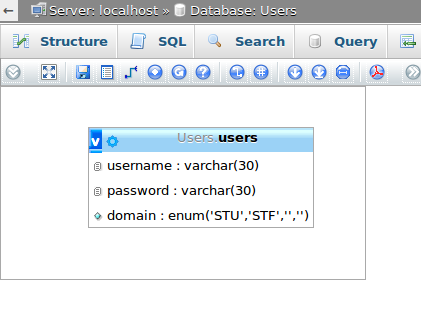
\includegraphics[width=10cm]{Users}
\caption{Users database and table }
\end{figure}
\end{center}

The possible improvement in this user database design would be storing the password as an encrypted password rather than storing it as is, this would be done to improve system security considering the confidentiality of the information stored within the students record/marks system.  
 
\item The student information, individual course information, course components and their percentage contribution form part of a student record database system. 

\begin{center}
\begin{figure}[h]
\centering
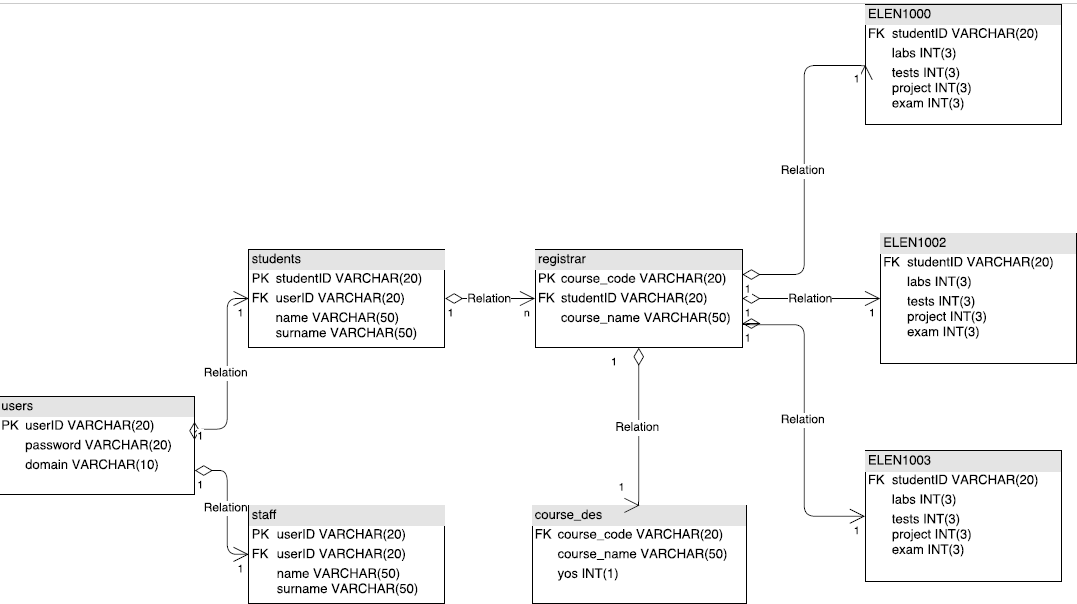
\includegraphics[width=14cm]{OverallDesign}
\caption{Student record Database design}
\end{figure}
\end{center}

\clearpage
\textbf{Students :}

This table is meant to store each individual student's information that include the student's name, surname and studentID which is a unique key that can be used to identify a student. This table has an auto incremented id as a primary key.  

\begin{center}
\begin{figure}[h]
\centering
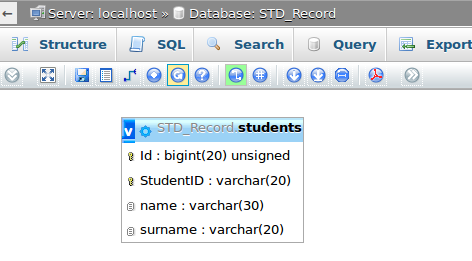
\includegraphics[width=10cm]{Students}
\caption{Students}
\end{figure}
\end{center}


\textbf{course$\_$description :}
This table contains the course code and course name, as the name suggests, it provides a description of each individual course in details. The course code is related to the course name in this table, each course code is unique and thus defined as such in the database.  

\textbf{registrar : }
This table is a logic table which is populated based on student registration business logic. This is specifically for student registration to a particular course, it constitute of a studentID and course$\_$code. On registration, the studentID is paired to a specific course$\_$code registered and the table's primary key is the id which is an auto incremented value.

\begin{center}
\begin{figure}[h]
\centering
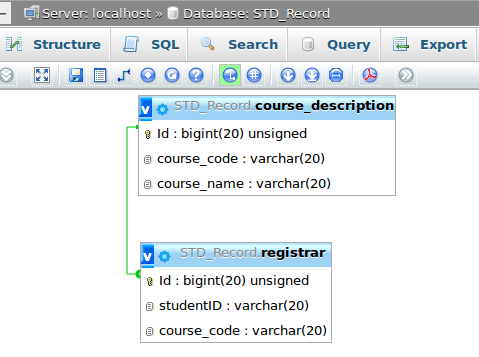
\includegraphics[width=8cm]{descriptionAndRegistar}
\caption{Course description and Registration}
\end{figure}
\end{center}

\clearpage
\textbf{staff : }
The staff table has a userID, this a unique variable, a staff name and surname as well as courses the lecture coordinates. An assumption that each individual lecture can not coordinate more than four courses was made to simplify the application due to implementation time constraint. However, an improvement in future versions would not make that assumption, instead lectures will be able to coordinate a non constant defined number of courses unless the business logic specifically require this to be the case.        

\begin{center}
\begin{figure}[h]
\centering
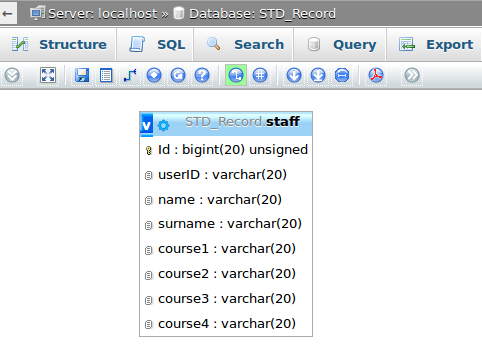
\includegraphics[width=8cm]{Staff}
\caption{Staff table}
\end{figure}
\end{center}

\textbf{courses : }
In order to simplify the problem due to time constraints, each course is designed to have its own individual table. This implementation however repeats information and does not take advantage of RDBMS special features that involve linking tables. This table would be improved in future versions of the application ensuring that there is no such a repetition which is redundant and limiting to the use of data stored.

This design was opted for in order to get a working prototype that can be demonstrated with ease. As the system grows, the design would make queering data a difficulty, and it would take more unnecessary time to query the database, shown below is a table example for an individual course

This table contains all course information that include course components and the marks to each of the components. Figure below shows the design for this table. 

\begin{center}
\begin{figure}[h]
\centering
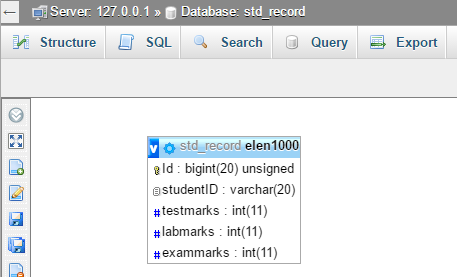
\includegraphics[width=8cm]{marks}
\caption{course table}
\end{figure}
\end{center}
  
\end{itemize}

\subsection{The application(Business model)}
PHP is  selected as a server scripting language. This language is chosen because of its simplicity, it is also a well documented programming language that is widely supported for web application development. Some of the required user interface specifications were not met due to time constraints and hence they will not be discussed in this report


\subsubsection{Logging in}
A php script file "login.php" is used to interact with the database. The login process is described below.

\begin{itemize}
\item Upon submission of the form from the user interface(UI), the credentials are posted to the login.php page and stored as variables.
\item A mysqli query is sent to the database requesting for the information in the table "users" of database "login" to be stored in an array. The array is a three-element array containing the user's id number, password and domain.
\item A while-loop is ran, using the query as the condition, to identify a match between the database array and the credentials saved from the form.
\item If-statements are used to condition redirecting of the client based on the match of the information and the domain that the user is meant to use.
\end{itemize}

Upon completion of logging in, a session is initiated and the user's id number is stored in the array for later usage.

The activity UML diagram of the logging-in process is demonstrated in the figure below.

\begin{center}
	\begin{figure}[h]
		\centering
		\includegraphics[width=8cm]{Login_activity}
		\caption{Activity UML diagram of the logging-in process}
	\end{figure}
\end{center} 

\subsubsection{Student}
From the given specifications, the student user-interface requirements include the displaying of all the course marks for every course the student registered for. This implemented the following way

\begin{itemize}
	\item Upon decision to check the marks, the user is redirected to a php script "marks\_helper.php". The user's student number is recalled from the session array and assigned to a variable.
	
	\item A mysqli query is ran as a condition to a while-loop. The query is meant to compare the student number from the session to the one obtained from the database table "registrar". Once matches are found, the "course\_code" that corresponds to the student number "registrar" table are, and the student number itself, are used to locate the marks in the relevant ELEN table.
	
	\item A while-loop is ran, using the query as the condition, is used to print out the relevant results to the user interface.
\end{itemize}

\subsubsection{School Administrator}
The accomplished implementation to the school administrator interface is the registration of a student to the database. For simplicity, it is assumed that the student is already registered to the login "users" table. This was implemented in the following manner:

\begin{itemize}
	\item Upon the choice to add a student after logging in, the administrator is prompted to input the name, surname, student number and course code of the student to be registered.
	\item The resulting form is posted to a php script "student\_register.php" and saved as variables for interaction with the database. Using a query, it is tested if the student number of the student can be matched to any other one in the database.  
	\item If the student number and course code posted to the page are tested for "registrar" table and not found, a query is made to add the values of the course code and student number to the "registrar" table.
	\item The student number is also, via a query, added to the relevant course that has been posted (should it exist).
\end{itemize}

subsubsection{Course co-ordinator}
From the given specifications, the course co-ordinator user-interface requirements include the displaying of all the students in a particular course and their respective marks. This is done in the following manner:

\begin{itemize}
	\item Once the course co-ordinator has selected to view the students and their marks, he will be prompted to input a course code for the course with which he is concerned.
	\item A form will be submitted to the page "marks.php" and the posted course code will be stored as a variable.
	\item A query is constructed as a while-loop argument to search for the table of the posted course code in the database "Student\_Records".
	\item If a match is found, the data of that particular table is saved in an array (one row at a time) and displayed to the user interface via the page "view\_marks.php"
\end{itemize}





